\chapter{Higher Order Corrections}
\section{Third Order in e Correction Terms}
Let us first look at a single contraction term in $S^{(3)}$:
\begin{equation}
N \left\{(\linktwoterms{\bar{\psi}}{ \cancel{A} \psi)_{x_{1}}(\bar{\psi}\cancel{A} }{\psi})_{x_{2}}(\bar{\psi}\cancel{A} \psi)_{x_{3}}\right\}
\end{equation}
One of the Feynmann diagrams for this would look like the following figure (\bluep{This is an unconnected diagram, not all lines are connected to one another in a single network})
\begin{figure}[H]
    \centering
\tikzset{every picture/.style={line width=0.75pt}} %set default line width to 0.75pt        

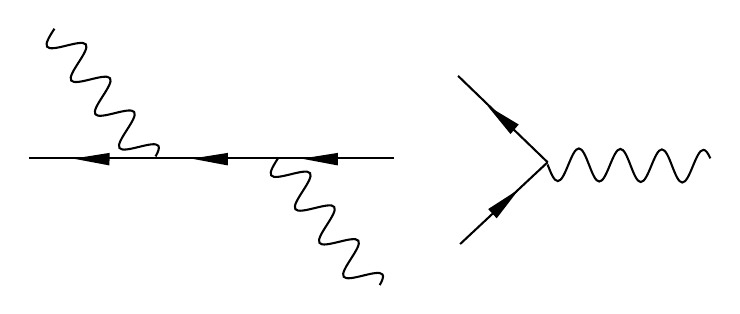
\begin{tikzpicture}[x=0.75pt,y=0.75pt,yscale=-1,xscale=1]
%uncomment if require: \path (0,300); %set diagram left start at 0, and has height of 300

%Straight Lines [id:da3780948069175081] 
\draw    (53,120) -- (228.87,120) ;
%Shape: Triangle [id:dp3960687992590355] 
\draw  [fill={rgb, 255:red, 0; green, 0; blue, 0 }  ,fill opacity=1 ] (134.43,120.3) -- (148.47,118.07) -- (148.4,122.93) -- cycle ;
%Shape: Triangle [id:dp05479485978100629] 
\draw  [fill={rgb, 255:red, 0; green, 0; blue, 0 }  ,fill opacity=1 ] (187.43,120.3) -- (201.47,118.07) -- (201.4,122.93) -- cycle ;
%Shape: Triangle [id:dp7557376074767396] 
\draw  [fill={rgb, 255:red, 0; green, 0; blue, 0 }  ,fill opacity=1 ] (77.43,120.3) -- (91.47,118.07) -- (91.4,122.93) -- cycle ;
%Shape: Wave [id:dp1885622709843502] 
\draw   (65.38,57.66) .. controls (63.03,61.35) and (60.79,64.86) .. (61.85,66.34) .. controls (62.9,67.81) and (66.95,66.83) .. (71.2,65.8) .. controls (75.45,64.76) and (79.5,63.78) .. (80.55,65.25) .. controls (81.61,66.73) and (79.37,70.24) .. (77.02,73.93) .. controls (74.66,77.62) and (72.42,81.13) .. (73.48,82.61) .. controls (74.53,84.08) and (78.58,83.1) .. (82.83,82.07) .. controls (87.08,81.03) and (91.13,80.05) .. (92.19,81.52) .. controls (93.24,83) and (91,86.51) .. (88.65,90.2) .. controls (86.29,93.89) and (84.06,97.4) .. (85.11,98.88) .. controls (86.16,100.35) and (90.21,99.37) .. (94.46,98.34) .. controls (98.71,97.3) and (102.76,96.32) .. (103.82,97.79) .. controls (104.87,99.27) and (102.63,102.78) .. (100.28,106.47) .. controls (97.92,110.16) and (95.69,113.67) .. (96.74,115.15) .. controls (97.79,116.62) and (101.84,115.64) .. (106.09,114.61) .. controls (110.34,113.57) and (114.4,112.59) .. (115.45,114.06) .. controls (116.15,115.05) and (115.39,116.94) .. (114.11,119.18) ;
%Shape: Wave [id:dp8210548245517799] 
\draw   (173.38,119.66) .. controls (171.03,123.35) and (168.79,126.86) .. (169.85,128.34) .. controls (170.9,129.81) and (174.95,128.83) .. (179.2,127.8) .. controls (183.45,126.76) and (187.5,125.78) .. (188.55,127.25) .. controls (189.61,128.73) and (187.37,132.24) .. (185.02,135.93) .. controls (182.66,139.62) and (180.42,143.13) .. (181.48,144.61) .. controls (182.53,146.08) and (186.58,145.1) .. (190.83,144.07) .. controls (195.08,143.03) and (199.13,142.05) .. (200.19,143.52) .. controls (201.24,145) and (199,148.51) .. (196.65,152.2) .. controls (194.29,155.89) and (192.06,159.4) .. (193.11,160.88) .. controls (194.16,162.35) and (198.21,161.37) .. (202.46,160.34) .. controls (206.71,159.3) and (210.76,158.32) .. (211.82,159.79) .. controls (212.87,161.27) and (210.63,164.78) .. (208.28,168.47) .. controls (205.92,172.16) and (203.69,175.67) .. (204.74,177.15) .. controls (205.79,178.62) and (209.84,177.64) .. (214.09,176.61) .. controls (218.34,175.57) and (222.4,174.59) .. (223.45,176.06) .. controls (224.15,177.05) and (223.39,178.94) .. (222.11,181.18) ;
%Straight Lines [id:da5687653686058063] 
\draw    (259.87,80.4) -- (303,122) ;
%Straight Lines [id:da8489603939248399] 
\draw    (303,122) -- (260.87,161.4) ;
%Shape: Triangle [id:dp4508463899972571] 
\draw  [fill={rgb, 255:red, 0; green, 0; blue, 0 }  ,fill opacity=1 ] (276.14,96.63) -- (288.32,103.93) -- (285.14,107.62) -- cycle ;
%Shape: Triangle [id:dp5269520777958134] 
\draw  [fill={rgb, 255:red, 0; green, 0; blue, 0 }  ,fill opacity=1 ] (287.09,136.96) -- (278.43,148.23) -- (275.13,144.65) -- cycle ;
%Shape: Wave [id:dp30185838683938926] 
\draw   (302.99,123.1) .. controls (304.57,127.18) and (306.09,131.06) .. (307.9,131.08) .. controls (309.71,131.1) and (311.31,127.25) .. (312.99,123.21) .. controls (314.66,119.17) and (316.27,115.32) .. (318.08,115.34) .. controls (319.89,115.36) and (321.4,119.25) .. (322.99,123.32) .. controls (324.57,127.4) and (326.09,131.28) .. (327.9,131.3) .. controls (329.71,131.33) and (331.31,127.48) .. (332.99,123.44) .. controls (334.66,119.4) and (336.27,115.55) .. (338.08,115.57) .. controls (339.88,115.59) and (341.4,119.47) .. (342.99,123.55) .. controls (344.57,127.63) and (346.09,131.51) .. (347.89,131.53) .. controls (349.7,131.55) and (351.31,127.71) .. (352.98,123.66) .. controls (354.66,119.62) and (356.26,115.78) .. (358.07,115.8) .. controls (359.88,115.82) and (361.4,119.7) .. (362.98,123.78) .. controls (364.57,127.86) and (366.08,131.74) .. (367.89,131.76) .. controls (369.7,131.78) and (371.31,127.93) .. (372.98,123.89) .. controls (374.66,119.85) and (376.26,116) .. (378.07,116.02) .. controls (379.28,116.04) and (380.36,117.77) .. (381.41,120.13) ;




\end{tikzpicture}
    \caption{Single Contraction term of $S^{(3)}$}
    \label{fig:single-contraction-S3}
\end{figure}
As mentioned in the previous chapter, the single vertex interaction is not physically possible as it produce off-shell photon. We conclude here that \redp{any possible term in $S^{(3)}$ that has a vertex factor $(\bar{\psi}\cancel{A}\psi)_{x_i}$ alone, unconnected to a contraction, is \textbf{not physical and can be ignored.}}

Let's look at one of three contraction term:
\begin{equation}
N \left\{(\UOLunderbr{\bar{\psi} \cancel{A} \overbracket{\psi)_{x_{1}}(\bar{\psi}}}[\cancel{A} \psi]\UOLunderbrl{)_{x_{2}}(\bar{\psi}\cancel{A}} \psi)_{x_{3}}\right\}
\end{equation}
A typical Feynman diagram for this looks like
\begin{figure}[H]
    \centering

\tikzset{every picture/.style={line width=0.75pt}} %set default line width to 0.75pt        

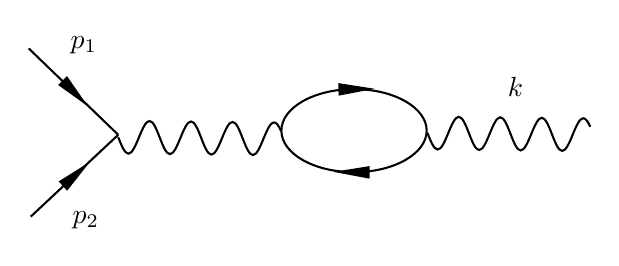
\begin{tikzpicture}[x=0.75pt,y=0.75pt,yscale=-1,xscale=1]
%uncomment if require: \path (0,300); %set diagram left start at 0, and has height of 300

%Straight Lines [id:da5687653686058063] 
\draw    (259.87,80.4) -- (303,122) ;
%Straight Lines [id:da8489603939248399] 
\draw    (303,122) -- (260.87,161.4) ;
%Shape: Triangle [id:dp4508463899972571] 
\draw  [fill={rgb, 255:red, 0; green, 0; blue, 0 }  ,fill opacity=1 ] (287.15,137.03) -- (278.34,148.18) -- (275.1,144.56) -- cycle ;
%Shape: Triangle [id:dp5269520777958134] 
\draw  [fill={rgb, 255:red, 0; green, 0; blue, 0 }  ,fill opacity=1 ] (286.34,106.19) -- (274.79,97.92) -- (278.26,94.5) -- cycle ;
%Shape: Wave [id:dp30185838683938926] 
\draw   (302.99,123.1) .. controls (304.57,127.18) and (306.09,131.06) .. (307.9,131.08) .. controls (309.71,131.1) and (311.31,127.25) .. (312.99,123.21) .. controls (314.66,119.17) and (316.27,115.32) .. (318.08,115.34) .. controls (319.89,115.36) and (321.4,119.25) .. (322.99,123.32) .. controls (324.57,127.4) and (326.09,131.28) .. (327.9,131.3) .. controls (329.71,131.33) and (331.31,127.48) .. (332.99,123.44) .. controls (334.66,119.4) and (336.27,115.55) .. (338.08,115.57) .. controls (339.88,115.59) and (341.4,119.47) .. (342.99,123.55) .. controls (344.57,127.63) and (346.09,131.51) .. (347.89,131.53) .. controls (349.7,131.55) and (351.31,127.71) .. (352.98,123.66) .. controls (354.66,119.62) and (356.26,115.78) .. (358.07,115.8) .. controls (359.88,115.82) and (361.4,119.7) .. (362.98,123.78) .. controls (364.57,127.86) and (366.08,131.74) .. (367.89,131.76) .. controls (369.7,131.78) and (371.31,127.93) .. (372.98,123.89) .. controls (374.66,119.85) and (376.26,116) .. (378.07,116.02) .. controls (379.28,116.04) and (380.36,117.77) .. (381.41,120.13) ;
%Shape: Ellipse [id:dp21378260759473022] 
\draw   (381.6,120) .. controls (381.6,108.95) and (397.27,100) .. (416.6,100) .. controls (435.93,100) and (451.6,108.95) .. (451.6,120) .. controls (451.6,131.05) and (435.93,140) .. (416.6,140) .. controls (397.27,140) and (381.6,131.05) .. (381.6,120) -- cycle ;
%Shape: Wave [id:dp07427295068477802] 
\draw   (451.99,121.1) .. controls (453.57,125.18) and (455.09,129.06) .. (456.9,129.08) .. controls (458.71,129.1) and (460.31,125.25) .. (461.99,121.21) .. controls (463.66,117.17) and (465.27,113.32) .. (467.08,113.34) .. controls (468.89,113.36) and (470.4,117.25) .. (471.99,121.32) .. controls (473.57,125.4) and (475.09,129.28) .. (476.9,129.3) .. controls (478.71,129.33) and (480.31,125.48) .. (481.99,121.44) .. controls (483.66,117.4) and (485.27,113.55) .. (487.08,113.57) .. controls (488.88,113.59) and (490.4,117.47) .. (491.99,121.55) .. controls (493.57,125.63) and (495.09,129.51) .. (496.89,129.53) .. controls (498.7,129.55) and (500.31,125.71) .. (501.98,121.66) .. controls (503.66,117.62) and (505.26,113.78) .. (507.07,113.8) .. controls (508.88,113.82) and (510.4,117.7) .. (511.98,121.78) .. controls (513.57,125.86) and (515.08,129.74) .. (516.89,129.76) .. controls (518.7,129.78) and (520.31,125.93) .. (521.98,121.89) .. controls (523.66,117.85) and (525.26,114) .. (527.07,114.02) .. controls (528.28,114.04) and (529.36,115.77) .. (530.41,118.13) ;
%Shape: Triangle [id:dp13296502270667654] 
\draw  [fill={rgb, 255:red, 0; green, 0; blue, 0 }  ,fill opacity=1 ] (409.6,139.9) -- (423.63,137.67) -- (423.56,142.53) -- cycle ;
%Shape: Triangle [id:dp9482730045827157] 
\draw  [fill={rgb, 255:red, 0; green, 0; blue, 0 }  ,fill opacity=1 ] (423.6,99.88) -- (409.64,102.55) -- (409.56,97.68) -- cycle ;

% Text Node
\draw (286.4,79) node    {$p_{1}$};
% Text Node
\draw (287.4,163) node    {$p_{2}$};
% Text Node
\draw (494.4,99) node    {$k$};


\end{tikzpicture}
    \caption{A Three Contraction Term of $S^{(3)}$}
    \label{fig:3-contraction-S3}
\end{figure}
Note that the net result of Fig.(\ref{fig:3-contraction-S3}) is similar to what we saw in the previous chapter, where a real electron and a real positron transmute into a single off-shell photon. Thus, it is unphysical too.
\begin{center}
    \tikzset{every picture/.style={line width=0.75pt}} %set default line width to 0.75pt 
\begin{tikzpicture}[x=0.75pt,y=0.75pt,yscale=-1,xscale=1]
%uncomment if require: \path (0,300); %set diagram left start at 0, and has height of 300

%Straight Lines [id:da307650809518932] 
\draw    (58,58.37) -- (158,158.37) ;
%Straight Lines [id:da4053696323117585] 
\draw    (158,158.37) -- (59.87,247.8) ;
%Shape: Wave [id:dp5998613246245391] 
\draw   (158,157.8) .. controls (162.14,161.39) and (166.11,164.8) .. (170.63,164.8) .. controls (175.16,164.8) and (178.99,161.39) .. (183,157.8) .. controls (187.01,154.21) and (190.84,150.8) .. (195.37,150.8) .. controls (199.89,150.8) and (203.85,154.21) .. (208,157.8) .. controls (212.14,161.39) and (216.11,164.8) .. (220.63,164.8) .. controls (225.16,164.8) and (228.99,161.39) .. (233,157.8) .. controls (237.01,154.21) and (240.84,150.8) .. (245.37,150.8) .. controls (249.89,150.8) and (253.85,154.21) .. (258,157.8) .. controls (262.14,161.39) and (266.11,164.8) .. (270.63,164.8) .. controls (275.16,164.8) and (278.99,161.39) .. (283,157.8) .. controls (287.01,154.21) and (290.84,150.8) .. (295.37,150.8) .. controls (299.89,150.8) and (303.85,154.21) .. (308,157.8) .. controls (312.14,161.39) and (316.11,164.8) .. (320.63,164.8) .. controls (325.16,164.8) and (328.99,161.39) .. (333,157.8) .. controls (333,157.8) and (333,157.8) .. (333,157.8) ;
%Shape: Triangle [id:dp4766081790625024] 
\draw  [fill={rgb, 255:red, 0; green, 0; blue, 0 }  ,fill opacity=1 ] (115.33,115.49) -- (97.69,104.32) -- (103.66,98.17) -- cycle ;
%Shape: Triangle [id:dp2439506934283957] 
\draw  [fill={rgb, 255:red, 0; green, 0; blue, 0 }  ,fill opacity=1 ] (101.73,210.33) -- (113.1,192.82) -- (119.17,198.86) -- cycle ;

% Text Node
\draw (86,61.37) node    {$p_{1}$};
% Text Node
\draw (88,244.37) node    {$p_{2}$};
% Text Node
\draw (256,134.37) node    {$k$};


\end{tikzpicture}
\end{center}
In similar fashion, we can show that \redp{every term in $S^{(3)}$ is unphysical and contributes zero to the transmission amplitude.}

\begin{qt}
    Feynman's rules ignore the factorial in the denominator of each term because those rules are applied to each topologically distinct diagram.
\end{qt}
\section{Fourth Order in e Correction Terms}